

\vspace{-0.25cm}
\section{Preliminaries on LMs and attention sink}
\vspace{-0.15cm}
% Let $f_{\theta}$ be an auto-regressive LLM with $L$ decoder layers. 

% Most mainstream LLMs adopt a decoder-only Transformer architecture for auto-regressive text generation. Typically, they employ multi-head self-attention (MHSA) together with a casual mask to compute the attention weights. 

Let $f_{\theta}$ be an auto-regressive LM with $L$ transformer decoder blocks and $\boldsymbol{X}\in \mathbb{R}^{T \times |\mathbb{V}|}:=\{\boldsymbol{x}_1\textrm{,}\,\boldsymbol{x}_2\textrm{,}\,\ldots\textrm{,}\,\boldsymbol{x}_T\}$ are the input tokens, where each token $\boldsymbol{x}_t$ is a one-hot encoding and $|\mathbb{V}|$ is the vocabulary size of tokenizer $\mathbb{V}$. The LM output is also a sequence $\boldsymbol{Y}\in \mathbb{R}^{T \times |\mathbb{V}|}:=\{\boldsymbol{y}_1\textrm{,}\, \boldsymbol{y}_2\textrm{,}\,\ldots\textrm{,}\, \boldsymbol{y}_T\}=f_{\theta}(\boldsymbol{X})$, where $\boldsymbol{y}_t$ represents the predicted logits of $p(\boldsymbol{x}_{t+1}|\boldsymbol{x}_{\leq t})$. 


\textbf{Transformer blocks.} In the forward pass, $\boldsymbol{X}$ is first embedded as $\boldsymbol{H}^{0} \in\mathbb{R}^{T\times d}:=\boldsymbol{X}\boldsymbol{W}_{E}+\boldsymbol{P}$,  where $\boldsymbol{W}_{E}\in \mathbb{R}^{|\mathbb{V}|\times d}$ is the learnable word embedding, $\boldsymbol{P}\in\mathbb{R}^{T\times d}$ is the positional embedding, and $d$ is the hidden dimension. We denote $\boldsymbol{H}^{l}\in \mathbb{R}^{T\times d}:=\{\boldsymbol{h}_1^{l}\textrm{,}\,\boldsymbol{h}_2^{l}\textrm{,}\,\ldots\textrm{,}\,\boldsymbol{h}_T^{l}\}\textrm{,}\,1\leq l\leq L$ to be the output of the $l$-th block. Each block comprises a multi-head self-attention (MHSA) operation and a feed-forward network (FFN). The block has either a pre-norm or post-norm structure according to the location of layer normalization (LN)~\citep{ba2016layernormalization,zhang2019root}. Most of LLMs consider a pre-norm block, as also shown in Figure~\ref{architecture}(\emph{Left}):
\begin{equation}\label{eq-pre-norm}
    \boldsymbol{H}^{l}=\textrm{FFN}(\textrm{LN}(\boldsymbol{O}^l + \boldsymbol{H}^{l-1})) +  \boldsymbol{O}^l + \boldsymbol{H}^{l-1}\textrm{,}\,\,\,\,\boldsymbol{O}^l=\textrm{MHSA}(\textrm{LN}(\boldsymbol{H}^{l-1}))\textrm{,}
\end{equation}
while the post-norm transformer block is
\begin{equation}
\boldsymbol{H}^{l}=\textrm{LN}\left(\textrm{FFN}(\textrm{LN}(\boldsymbol{O}^l + \boldsymbol{H}^{l-1})) + \textrm{LN}(\boldsymbol{O}^l + \boldsymbol{H}^{l-1})\right)\textrm{,}\,\,\,\,\boldsymbol{O}^l=\textrm{MHSA}(\boldsymbol{H}^{l-1})\textrm{.}
\end{equation}

\begin{figure}[t]
\centering
\vspace{-1.1cm}
 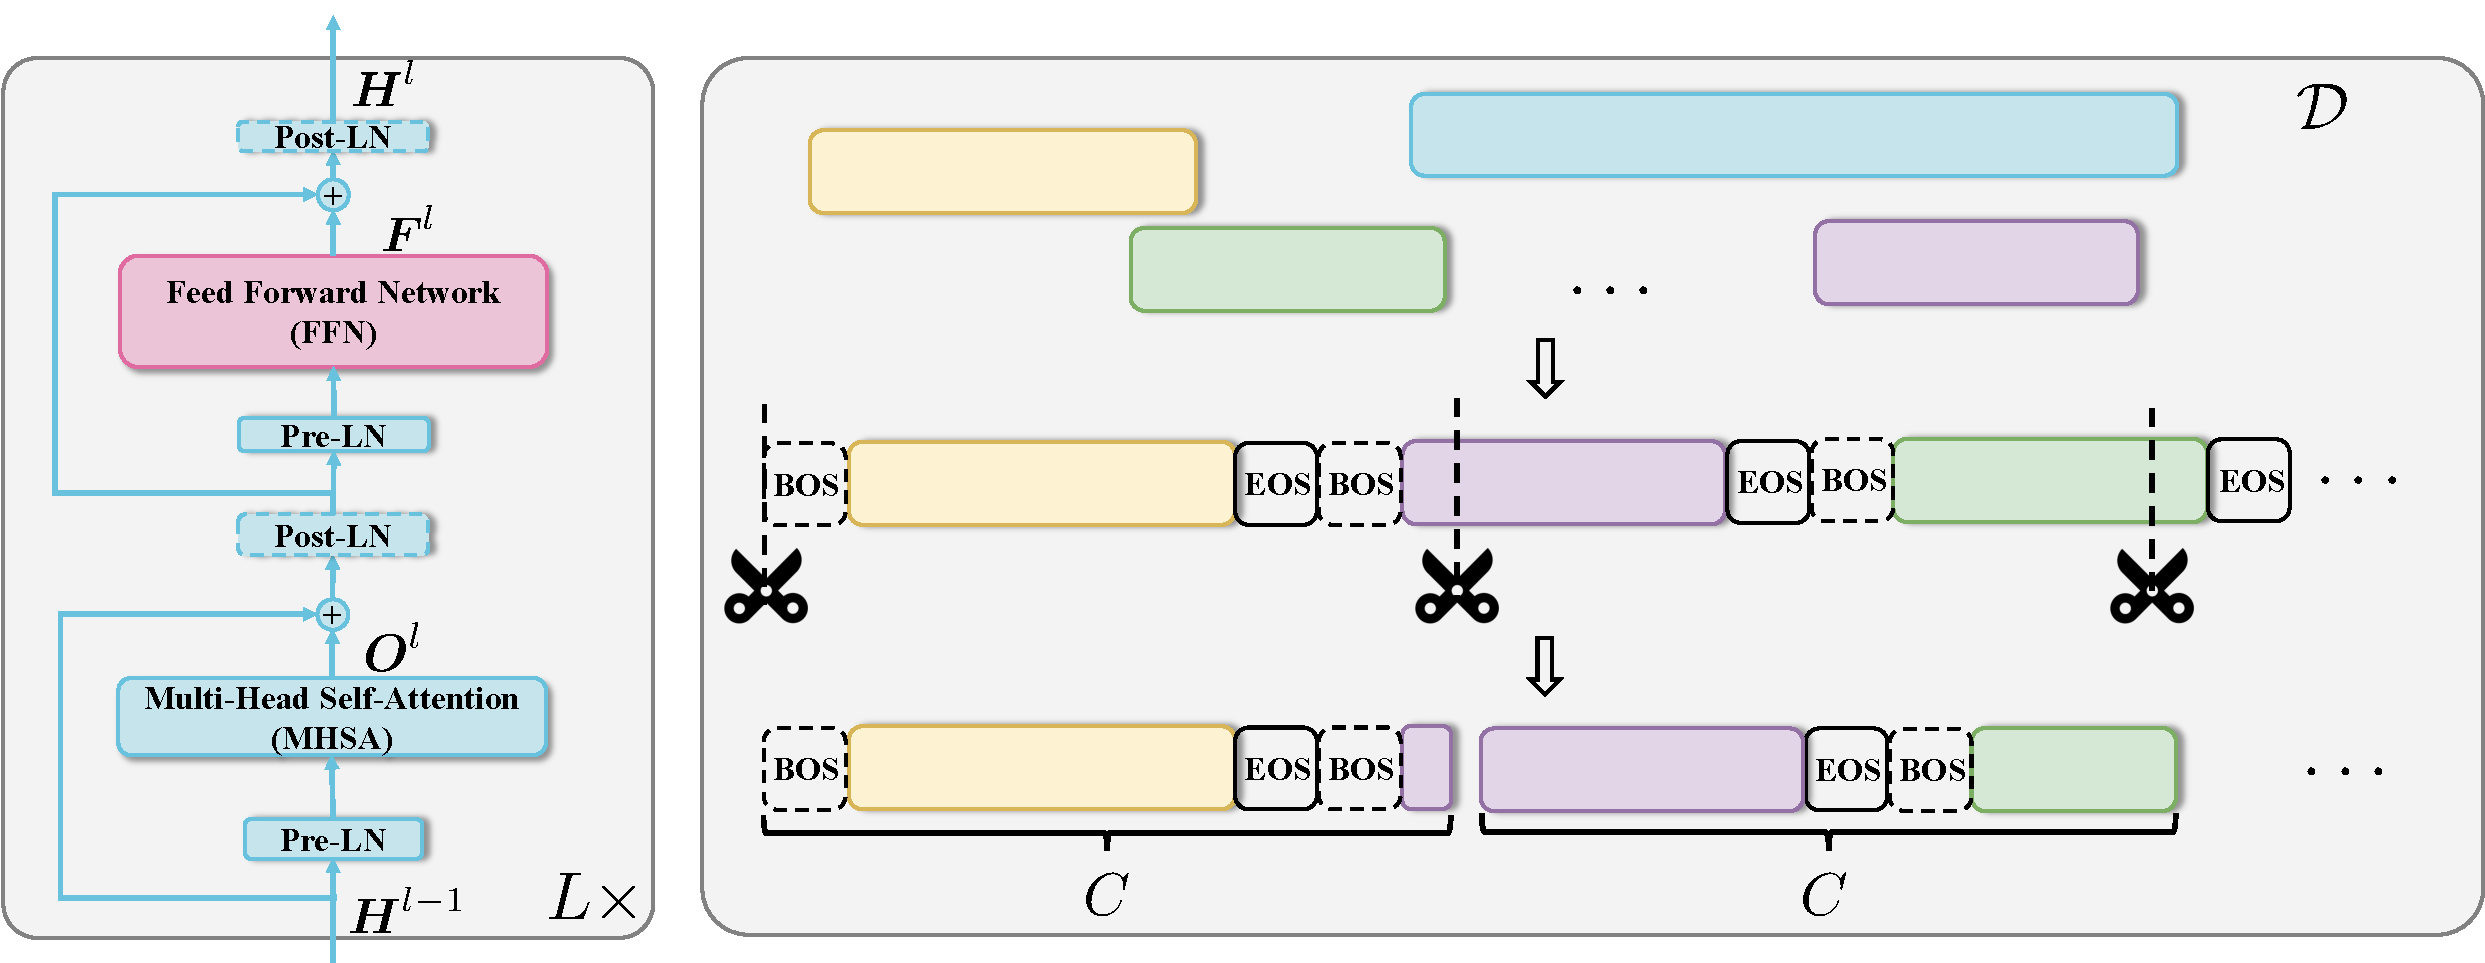
\includegraphics[width=\textwidth]{figures/architecture.pdf}
% \subfigure[]{\includegraphics[width=0.45\textwidth]{figures/domains_metric1.pdf}}
% \begin{subfigure}[t]{0.33\textwidth}
%     \centering
%     \includegraphics[width=\textwidth]{figures/pre-norm.pdf}
% \end{subfigure}
% \hfill
% \begin{subfigure}[t]{0.62\textwidth}
%     \centering
%     \includegraphics[width=\textwidth]{figures/pretrain.pdf}
% \end{subfigure}
\vspace{-0.6cm}
\caption{(\emph{Left}) Architecture of pre-norm transformer block (we highlight the location of post-norm LN using dashed lines). We denote the output of MHSA as $\boldsymbol{O}^l$ and the output of FFN as $\boldsymbol{F}^l$. (\emph{Right}) The packing strategy in the LM pre-training. All documents are concatenated with BOS (optional) and EOS tokens as the boundaries. Then it is chunked into equal-sized sequences with context length $C$.\looseness=-1
}
\vspace{-0.3cm}
\label{architecture}
\end{figure}

\textbf{MHSA layers.} In the MHSA layer, the input $\boldsymbol{H}^{l-1}$ are first transformed into keys, queries, and values: $\boldsymbol{K}^{l\textrm{,}h}=\boldsymbol{H}^{l-1}\boldsymbol{W}_{K}^{l\textrm{,}h}$, $\boldsymbol{Q}^{l\textrm{,}h}=\boldsymbol{H}^{l-1}\boldsymbol{W}_{Q}^{l\textrm{,}h}$, $\boldsymbol{V}^{l\textrm{,}h}=\boldsymbol{H}^{l-1}\boldsymbol{W}_{V}^{l\textrm{,}h}$ for each head $1\leq h\leq H$ (we omit the notation of LN when considering pre-norm design for simplicity). Here $\boldsymbol{W}_{K}^{l\textrm{,}h}, \boldsymbol{W}_{Q}^{l\textrm{,}h}, \boldsymbol{W}_{V}^{l\textrm{,}h} \in \mathbb{R}^{d\times d_h}\textrm{,}\,d_h=d/H$. Then the attention output is computed as
\begin{equation}
    \boldsymbol{A}^{l\textrm{,}h}= \textrm{Softmax}\big({\boldsymbol{Q}^{l\textrm{,}h}{\boldsymbol{K}^{l\textrm{,}h}}^\top}/{\sqrt{d_h}}+ \boldsymbol{M}\big)\textrm{,}\,\,\,\,
\boldsymbol{O}^l=\textrm{Concat}_{h=1}^H\left(\boldsymbol{A}^{l\textrm{,}h}\boldsymbol{V}^{l\textrm{,}h}\right)\boldsymbol{W}_{O}^l\textrm{,}
\end{equation}
where $\boldsymbol{M}\in \mathbb{R}^{T\times T}$ is an attention mask. For vanilla causal attention, $\boldsymbol{M}_{ij}=-\infty$ for $i<j$ and $\boldsymbol{M}_{ij}=0$ for $i\geq j$. Finally, the output of final transformer block $\boldsymbol{H}^{L}$ is fed into an unembedding layer for prediction: $\boldsymbol{Y}=\textrm{LN}(\boldsymbol{H}^{L})\boldsymbol{W}_{\textrm{cls}}$, where $\boldsymbol{W}_{\textrm{cls}}\in\mathbb{R}^{d\times |\mathbb{V}|}$.\looseness=-1

\textbf{Positional embedding.} NoPE~\citep{kazemnejad2024impact} considered no explicit positional embedding (PE) in LMs, where $\boldsymbol{P}=\boldsymbol{0}$. When using absolute PE~\citep{vaswani2017attention}, $\boldsymbol{P}$ is a periodic function of token positions. \citet{devlin2019bert,Brown2020language} adopted a learnable PE, which means $\boldsymbol{P}$ is a learnable embedding of token positions. The dot product between each query and key meets $\langle\boldsymbol{q}_i\textrm{,}\, \boldsymbol{k}_j\rangle=\boldsymbol{q}_i \boldsymbol{k}_j^\top$ when using the above three PEs. While for relative PE~\citep{raffel2020exploring}, ALiBi~\citep{press2021train}, Rotary~\citep{su2024roformer}, they have  $\boldsymbol{P}=\boldsymbol{0}$. Instead, they modify the dot product $\langle\boldsymbol{q}_i\textrm{,}\, \boldsymbol{k}_j\rangle$. For relative PE and ALiBi, $\langle\boldsymbol{q}_i\textrm{,}\, \boldsymbol{k}_j\rangle=\boldsymbol{q}_i \boldsymbol{k}_j^\top + g(i-j)$, where $g(\cdot)$ is pre-defined function of the distance between two token positions. For Rotary, $\langle\boldsymbol{q}_i\textrm{,}\, \boldsymbol{k}_j\rangle=\boldsymbol{q}_i\boldsymbol{R}_{\Theta\textrm{,}\,j-i} \boldsymbol{k}_j^\top$, where $\boldsymbol{R}_{\Theta\textrm{,}\,(\cdot)}$ is a pre-defined rotation matrix. We include detailed formulations of the above PEs in Appendix~\ref{appendix_llm}.\looseness=-1


\textbf{Auto-regressive objective.}  The pre-training objective of LMs is to maximize the likelihood of input data: $\theta^*=\arg\max_{\theta} \mathbb{E}_{\boldsymbol{X}\sim p_{\textrm{data}}}\left[\sum_{t=1}^T\log p_{\theta}(\boldsymbol{x}_t|\boldsymbol{x}_{<t})\right]$, where $p_{\textrm{data}}$ refers to the data distribution. 



% $\boldsymbol{X}=\{\boldsymbol{x}_1\textrm{,}\,\boldsymbol{x}_2\textrm{,}\,\ldots\textrm{,}\,\boldsymbol{x}_T\}$, where $\boldsymbol{X}\sim p_{\textrm{data}}$ and $p_{\textrm{data}}$ refers to data distribution. Then the auto- represented as an optimization problem: $\theta^*=\arg\max_{\theta} \mathbb{E}_{\boldsymbol{X}\sim p_{\textrm{data}}}\left[\sum_{t=1}^T\log p_{\theta}(\boldsymbol{x}_t|\boldsymbol{x}_{<t})\right]$.

% \begin{equation}
%     \theta^*=\arg\max_{\theta} \mathbb{E}_{\boldsymbol{X}\sim p_{\textrm{data}}}\left[\sum_{t=1}^T\log p_{\theta}(\boldsymbol{x}_t|\boldsymbol{x}_{<t})\right]\textrm{.}
% \end{equation}

% \begin{equation}
%     \theta^*=\mathcal{L}(l\,\textrm{;}\,\theta\,\textrm{;}\,\Phi)\textrm{,}\,\,\,\,l= \arg\max\mathbb{E}_{\boldsymbol{X}\sim\boldsymbol{P}}\left\{\sum_{t=1}^T\log p_{\theta}(\boldsymbol{x}_t|\boldsymbol{x}_{<t})\right\}
% \end{equation}

% Therefore, the trained LLMs are highly related to the model parameterization $\theta$, data distribution $\boldsymbol{p}_{\textrm{data}}$, the auto-regressive training objective, and the optimization algorithm.

\textbf{Packing documents in pre-training.} Given a large corpus $\mathcal{D}=\{\boldsymbol{d}_1\textrm{,}\,\boldsymbol{d}_2\textrm{,}\,\cdots\textrm{,}\,\boldsymbol{d}_{|\mathcal{D}|}\}$, where each $\boldsymbol{d}_i$ represents a document containing a sequence of tokens. A packing strategy is adopted in the LM pre-training, as present in Figure~\ref{architecture}(\emph{Right}). All documents are concatenated and chunked into sequences with a context length of $C$. Each chunk could start with any token within one document or the BOS/EOS token. Then the empirical loss function for each chunk is $\mathcal{L}=\sum_{t=2}^C\log p_{\theta}(\boldsymbol{x}_t|\boldsymbol{x}_{<t})$. We note that $p_{\theta}(\boldsymbol{x}_1)$ is ignored since $\boldsymbol{y}_1=f_{\theta}(\boldsymbol{x}_1)$ is the prediction for the next token $\boldsymbol{x}_2$.\looseness=-1


% If there are no BOS tokens in the pre-training, BOS token will be the same as EOS token during the inference. 


\textbf{LM inference.} During the inference, a BOS token is fed into the model as the prefix for unconditional generation: $\boldsymbol{x}'_t\sim p_{\theta}(\boldsymbol{x}'_t|\boldsymbol{x}'_{<t}\textrm{,}\,\boldsymbol{x}\textrm{,}\,\textrm{BOS})$, where $\boldsymbol{x}'_t$ is the $t$-th generated token, $\boldsymbol{x}$ is the optional prompt. If there are no BOS tokens in the pre-training, the EOS token is considered as the BOS.\looseness=-1


% , results in $\theta^*=\arg\max_{\theta} \sum_{t=2}^T\log p_{\theta}(\boldsymbol{x}_t|\boldsymbol{x}_{<t})$. To enable the supervision of $p_{\theta}(\boldsymbol{x}_1)$, the normal practice is to introduce a BOS (beginning of sequence) token before $\boldsymbol{x}_1$ for each data sample, resulting in $\theta^*=\arg\max_{\theta} \sum_{t=1}^T\log p_{\theta}(\boldsymbol{x}_t|\boldsymbol{x}_{<t}\textrm{,}\,\, \textrm{BOS})$.



% where $T$ is the number of tokens and $d$ is the hidden dimension. The attention weights $\boldsymbol{A}_h^{(l)}\in \mathbb{R}^{T\times T}$ for $l$-th layer $h$-th head can be computed


% where $\boldsymbol{Q}_{h}^{(l)}$ and $\boldsymbol{K}_{h}^{(l)}$ are projection layers to transform the input sequence into queries and keys, and $d'=\frac{d}{H}$ denotes the hidden dimension for each head. Considering the causal mask used during the computation of attention weights, $\boldsymbol{A}_h^{(l)}$ should be a lower triangle matrix with ${\boldsymbol{A}_h^{(l)}}_{i, i+1:T}=0\textrm{,}\,\, \textrm{for}\,\,1\leq i \leq T$. 

\textbf{Attention sink.} \citet{xiao2023efficient} revealed that LLMs allocate significant attention scores to specific token positions, e.g. the first token (not necessary to be a BOS token), resulting in ``vertical'' attention patterns. To represent this, we have the attention scores $\boldsymbol{A}_{i\textrm{,}\,1}^{l\textrm{,}\,h}\gg \textrm{mean}(\boldsymbol{A}_{i\textrm{,}\,j\neq 1}^{l\textrm{,}\,h})$.\looseness=-1


% \citet{sun2024massive} observed that attention sink is correlated to the \textit{massive activations} of hidden states $\boldsymbol{H}^l$ in LLMs. They showed that the hidden states of sink tokens, e.g., $\boldsymbol{h}_1^l$, typically exhibit huge magnitude in several dimensions.



% To represent this using notations, we first consider the average attention weights. When LLMs allocate the same attention weights to each token position
% \begin{equation}
%     \boldsymbol{\hat{A}}_{i,j}^{l,h}=\left\{
%     \begin{array}{lcl}
%         1/i & &\textrm{for} \,\,\,\, 1 \leq i \leq T \textrm{,}\,\,\,\, 1 \leq j \leq i \\
%         0 && \textrm{for} \,\,\,\, 1 \leq i \leq T \textrm{,}\,\,\,\,  i < j 
%     \end{array}
%     \right.
% \end{equation}

% If $k$-th token position is an attention sink, it should be $\sum_{i=k}^T\boldsymbol{A}^{l,h}_{i,k}\gg \sum_{i=k}^T\boldsymbol{\hat{A}}^{l,h}_{i,k}$.\looseness=-1

% Most literature~\citep{xiao2023efficient} considers attention sink existing in the initial token, which shows a strong position association. While \citet{yu2024unveiling} argue that attention sink could also exist in other token positions. However, these non-initial high-attention tokens have no specific positions. Considering the intriguing property of the above position association, we focus on the initial token attention sink in this paper.\looseness=-1

% and its application potential in cache optimization and long context scenarios



% and $\boldsymbol{X}=\{\boldsymbol{x}_1, \boldsymbol{x}_2, ..., \boldsymbol{x}_T\}$ to be the input tokens.


% Let $f_{\theta}$ be a Transformer with $L$ decoder layers and $\boldsymbol{X}=\{\boldsymbol{x}_1, \boldsymbol{x}_2, ..., \boldsymbol{x}_T\}$ to be the input tokens. Typically, $f_{\theta}$ will demonstrate attention sink scenario, where attention weights for each token position concentrate on the initial token.